\documentclass[
  parskip=half,           % halbzeiliger Zeileneinzug nach Absatz
  bibliography=totoc,     % Literatur im Inhaltsverzeichnis
  captions=tableheading,  % Tabellenüberschriften
  titlepage=firstiscover, % Titelseite ist Deckblatt
]{scrartcl}

\usepackage{listings}
\lstdefinestyle{customc}{
  belowcaptionskip=1\baselineskip,
  breaklines=true,
  frame=L,
  xleftmargin=\parindent,
  language=C,
  showstringspaces=false,
  basicstyle=\footnotesize\ttfamily,
  keywordstyle=\bfseries\color{green!40!black},
  commentstyle=\itshape\color{purple!40!black},
  identifierstyle=\color{blue},
  stringstyle=\color{orange},
}

\lstdefinestyle{customasm}{
  belowcaptionskip=1\baselineskip,
  frame=L,
  xleftmargin=\parindent,
  language=[x86masm]Assembler,
  basicstyle=\footnotesize\ttfamily,
  commentstyle=\itshape\color{purple!40!black},
}
\lstset{language=Python}
\lstset{escapechar=@,style=customc}

\usepackage{geometry}
\geometry{a4paper,left=25mm,right=25mm, top=3cm, bottom=3cm}

% Paket float verbessern
\usepackage{scrhack}

% Warnung, falls nochmal kompiliert werden muss
\usepackage[aux]{rerunfilecheck}

% deutsche Spracheinstellungen
\usepackage{polyglossia}
\setmainlanguage{german}

% unverzichtbare Mathe-Befehle
\usepackage{amsmath}
% viele Mathe-Symbole
\usepackage{amssymb}
% Erweiterungen für amsmath
\usepackage{mathtools}

% Fonteinstellungen
\usepackage{fontspec}
% Latin Modern Fonts werden automatisch geladen

\usepackage[
  math-style=ISO,    % ┐
  bold-style=ISO,    % │
  sans-style=italic, % │ ISO-Standard folgen
  nabla=upright,     % │
  partial=upright,   % ┘
  warnings-off={           % ┐
    mathtools-colon,       % │ unnötige Warnungen ausschalten
    mathtools-overbracket, % │
  },                       % ┘
]{unicode-math}

% traditionelle Fonts für Mathematik
\setmathfont{Latin Modern Math}
\setmathfont{XITS Math}[range={scr, bfscr}]
\setmathfont{XITS Math}[range={cal, bfcal}, StylisticSet=1]

% Zahlen und Einheiten
\usepackage[
  locale=DE,                 % deutsche Einstellungen
  separate-uncertainty=true, % immer Fehler mit \pm
  per-mode=reciprocal,       % ^-1 für inverse Einheiten
  % alternativ:
  % per-mode=reciprocal, % m s^{-1}
  % decimal-marker=., % . statt , f�r Dezimalzahlen
]{siunitx}

% chemische Formeln
\usepackage[
  version=4,
  math-greek=default, % ┐ mit unicode-math zusammenarbeiten
  text-greek=default, % ┘
]{mhchem}

% richtige Anführungszeichen
\usepackage[autostyle]{csquotes}

% schöne Brüche im Text
\usepackage{xfrac}

\usepackage{blindtext}    % \blindtext zum Testen von Texten.

% Standardplatzierung für Floats einstellen
\usepackage{float}
\floatplacement{figure}{htbp}
\floatplacement{table}{htbp}

% Floats innerhalb einer Section halten
\usepackage[
  section, % Floats innerhalb der Section halten
  below,   % unterhalb der Section aber auf der selben Seite ist ok
]{placeins}

% Seite drehen für breite Tabellen
\usepackage{pdflscape}

% mehrere Seiten einer einzelnen pdf, zB
% 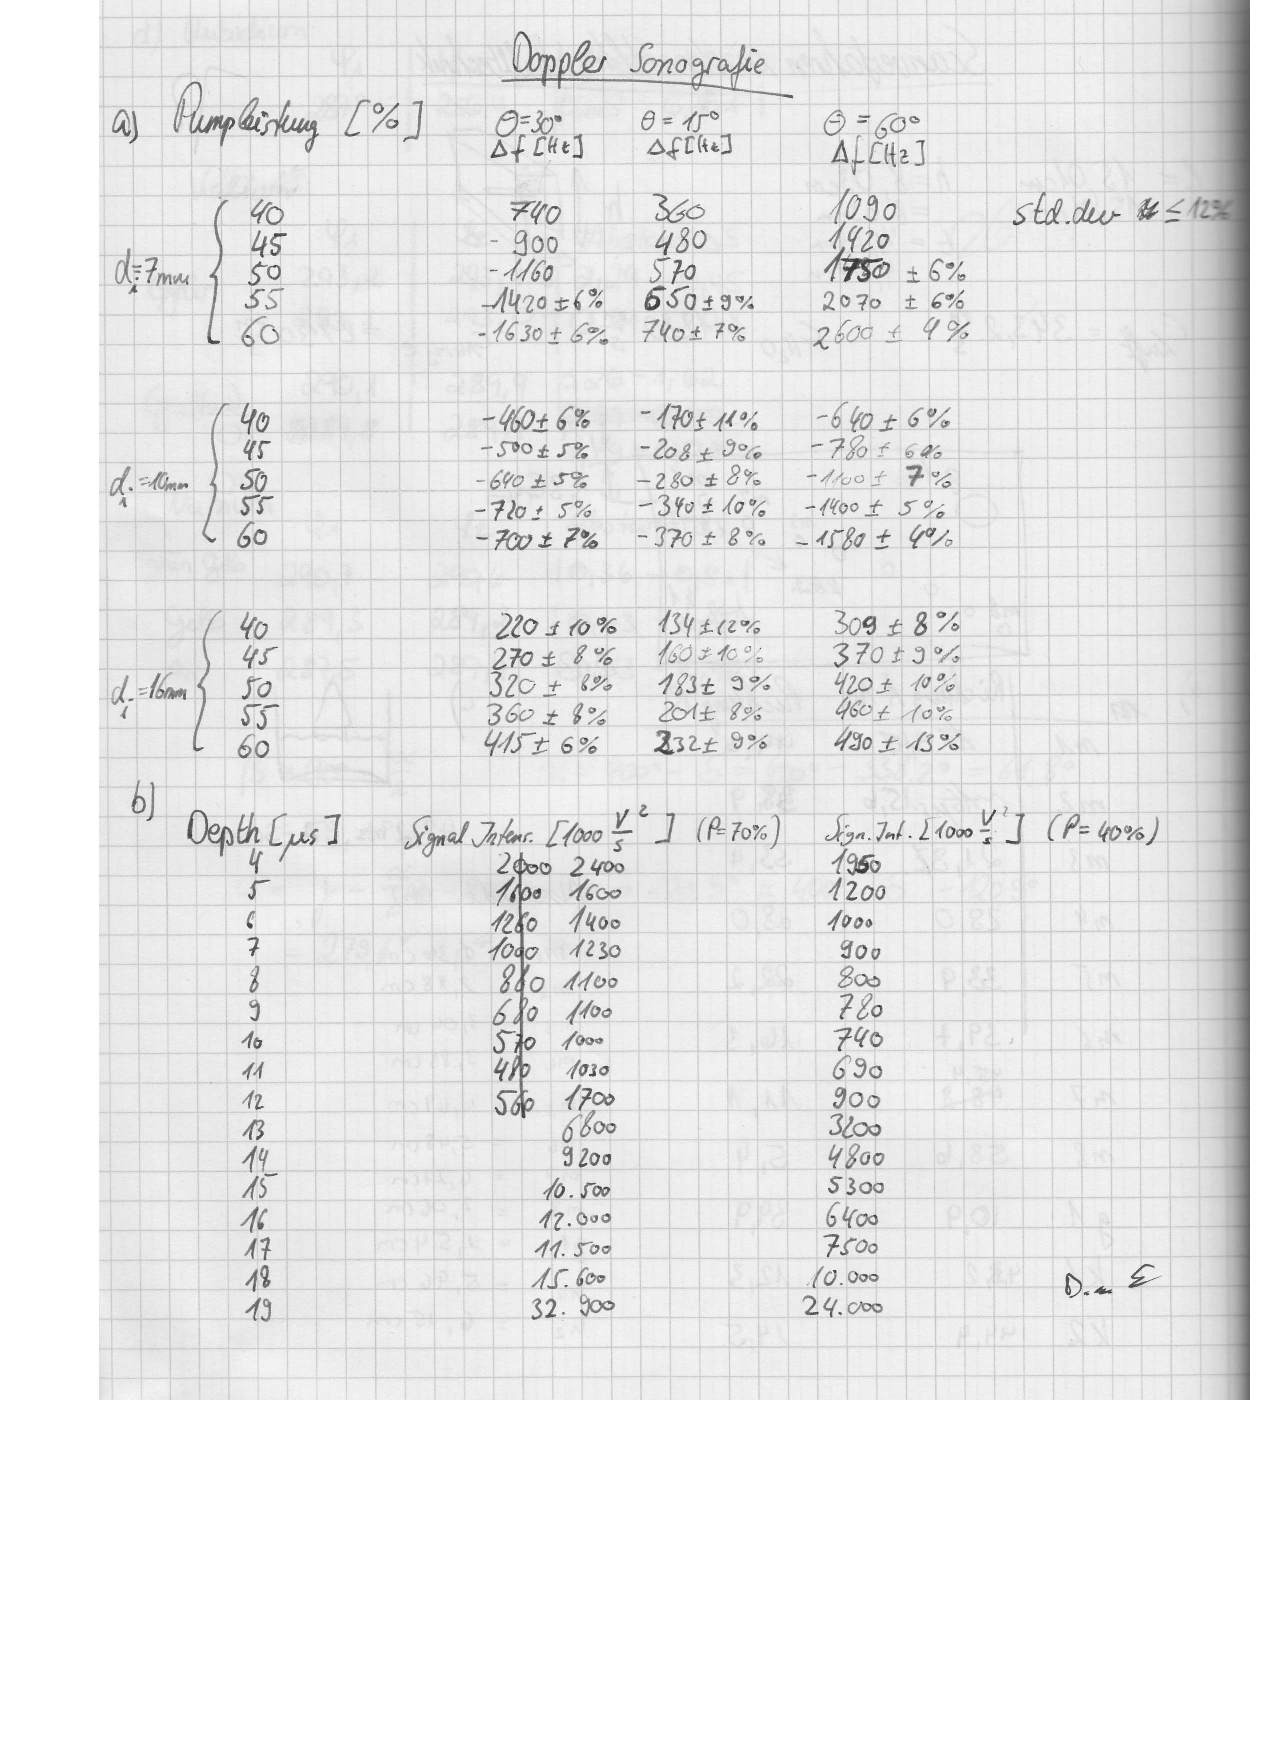
\includepdf[pages={1-2}]{Bilder/Messdaten.pdf}
\usepackage{pdfpages}

% Captions schöner machen.
\usepackage[
  labelfont=bf,        % Tabelle x: Abbildung y: ist jetzt fett
  font=small,          % Schrift etwas kleiner als Dokument
  width=0.9\textwidth, % maximale Breite einer Caption schmaler
  %indention=1cm        % Einrückung nach der ersten Zeile
]{caption}
% subfigure, subtable, subref
\usepackage{subcaption}

% mit Buchstabend gelistete items: \begin{enumerate}[label={\alph*)}]
\usepackage{enumitem}

% Grafiken können eingebunden werden
\usepackage{graphicx}
% größere Variation von Dateinamen möglich (Probleme mit Leerzeichen behoben)
\usepackage{grffile}

% schöne Tabellen
\usepackage{booktabs}
\sisetup{table-format=1.2}
%\begin{tabular}{S[table-format=3.0] S S S S[table-format=3.2]}
%table-format : 3 stellen vor, 0 stellen nach dem Komma
% S steht f�r siunix, dh. wir verwenden solche Zahlen
% \multicolumn{2}{c}{Spalte 1}
% wie in excel Spalten zusammenf�gen
% Einheiten: {$\lambda \:/\: \si{\nano\meter}$}

% Uncertainties:
%\begin{tabular}{
% S[table-format=3.1]
% @{${}\pm{}$}
% S[table-format=2.1]
% }
% \toprule
% \multicolumn{2}{c}{$x \:/\: \si{\ohm}$} \\
% \midrule
% 632.4 & 5.7 \\

% Verbesserungen am Schriftbild
\usepackage{microtype}

% Literaturverzeichnis
\usepackage[
  backend=biber,
]{biblatex}
% Quellendatenbank
\addbibresource{Quellen.bib}
\addbibresource{programme.bib}

% Hyperlinks im Dokument
\usepackage[
  unicode,        % Unicode in PDF-Attributen erlauben
  pdfusetitle,    % Titel, Autoren und Datum als PDF-Attribute
  pdfcreator={},  % ┐ PDF-Attribute säubern
  pdfproducer={}, % ┘
  linkcolor=blue, % einfache interne Verkn?pfungen
  citecolor=blue, % Verweise auf Literaturverzeichniseintr?ge im Text
]{hyperref}
% erweiterte Bookmarks im PDF
\usepackage{bookmark}

% Trennung von Wörtern mit Strichen
\usepackage[shortcuts]{extdash}


% TYPOGRAPHIE:

% Nutze z.\,B. um Zeilenumbruch zu verhindern.
% Gedankenstriche mit --  (statt -)
% \\[2\baselineskip] erstellt einen vspace mit 2 Baselines, also 2 Zeilen


% \renewcommand{\baselinestretch}{1.3}										%Zeilenabstand


% zu breite Tabellen/Figures:
%\OverfullCenter{
%  \begin{figure}
%   ...
%  \end{figure}
%}
\NewDocumentCommand \OverfullCenter {+m} {
  \noindent\makebox[\linewidth]{#1} }



% Klammern werden nach außen hin leicht größer gesetzt.
\setlength{\delimitershortfall}{-1sp}



\begin{document}
  \begin{figure*}
      \centering
      \begin{subfigure}[b]{0.31\textwidth}
          \centering
          \includegraphics[width=\textwidth]{build/u11.pdf}
          \caption*%
          {{\small $u_{1,1}$}}
      \end{subfigure}
      \hfill
      \begin{subfigure}[b]{0.31\textwidth}
          \centering
          \includegraphics[width=\textwidth]{build/u12.pdf}
          \caption*%
          {{\small $u_{1,2}$}}
      \end{subfigure}
      \hfill
      \begin{subfigure}[b]{0.31\textwidth}
          \centering
          \includegraphics[width=\textwidth]{build/u13.pdf}
          \caption*%
          {{\small $u_{1,3}$}}
      \end{subfigure}
      \vskip\baselineskip
      \begin{subfigure}[b]{0.31\textwidth}
          \centering
          \includegraphics[width=\textwidth]{build/u21.pdf}
          \caption*%
          {{\small $u_{2,1}$}}
      \end{subfigure}
      \quad
      \begin{subfigure}[b]{0.31\textwidth}
          \centering
          \includegraphics[width=\textwidth]{build/u22.pdf}
          \caption*%
          {{\small $u_{2,2}$}}
      \end{subfigure}
      \quad
      \begin{subfigure}[b]{0.31\textwidth}
          \centering
          \includegraphics[width=\textwidth]{build/u23.pdf}
          \caption*%
          {{\small $u_{2,3}$}}
      \end{subfigure}
      \vskip\baselineskip
      \begin{subfigure}[b]{0.31\textwidth}
          \centering
          \includegraphics[width=\textwidth]{build/u31.pdf}
          \caption*%
          {{\small $u_{3,1}$}}
      \end{subfigure}
      \quad
      \begin{subfigure}[b]{0.31\textwidth}
          \centering
          \includegraphics[width=\textwidth]{build/u32.pdf}
          \caption*%
          {{\small $u_{3,2}$}}
      \end{subfigure}
      \quad
      \begin{subfigure}[b]{0.31\textwidth}
          \centering
          \includegraphics[width=\textwidth]{build/u33.pdf}
          \caption*%
          {{\small $u_{3,3}$}}
      \end{subfigure}
      \caption[]
      {Eigenmoden der halben Trommel.}
  \end{figure*}
\end{document}


% % Examples
% \begin{equation}
%   U(t) = a \sin(b t + c) + d
% \end{equation}
%
% \begin{align}
%   a &= \input{a.tex} \\
%   b &= \input{b.tex} \\
%   c &= \input{c.tex} \\
%   d &= \input{d.tex} .
% \end{align}
% Die Messdaten und das Ergebnis des Fits sind in Abbildung~\ref{fig:plot} geplottet.
%
% %Tabelle mit Messdaten
% \begin{table}
%   \centering
%   \caption{Messdaten.}
%   \label{tab:data}
%   \sisetup{parse-numbers=false}
%   \begin{tabular}{
%     S[table-format=1.3]
%     S[table-format=-1.2]
%     @{${}\pm{}$}
%     S[table-format=1.2]
%     @{\hspace*{3em}\hspace*{\tabcolsep}}
%     S[table-format=1.3]
%     S[table-format=-1.2]
%     @{${}\pm{}$}
%     S[table-format=1.2]
%   }
%     \toprule
%     {$t \:/\: \si{\milli\second}$} & \multicolumn{2}{c}{$U \:/\: \si{\kilo\volt}$\hspace*{3em}} &
%     {$t \:/\: \si{\milli\second}$} & \multicolumn{2}{c}{$U \:/\: \si{\kilo\volt}$} \\
%     \midrule
%     1.7 & 10 \\
2.3 & 20 \\
3.5 & 30 \\
4.4 & 40 \\

%     \bottomrule
%   \end{tabular}
% \end{table}
%
% % Standard Plot
% \begin{figure}
%   \centering
%   \includegraphics{plot.pdf}
%   \caption{Messdaten und Fitergebnis.}
%   \label{fig:plot}
% \end{figure}
